\documentclass{article}
\usepackage[utf8]{inputenc}
\textheight = 25cm 
\textwidth = 15cm
\topmargin = -2.5cm 
\oddsidemargin = 1.5cm
\usepackage{float}
\usepackage{graphicx}
\graphicspath{{./images/}}

\usepackage{amsmath}
\usepackage{mathtools, xparse}
\usepackage[shortlabels]{enumitem}
\usepackage[most]{tcolorbox}
\usepackage{adjustbox}
\usepackage{bm} 

\DeclarePairedDelimiter{\norm}{\lVert}{\rVert}

\title{Tarea 7 Mecánica Analítica}
\author{Cerritos Lira Carlos}
\date{21 de Abril del 2020}

\begin{document}
\maketitle
\section*{Problemas}
\section*{1.-}
\subsection*{5.2)}
Utilizar el resultado del problema 5-1 para hallar las ecuaciones de
Lagrange de una partícula cuya energía cinética es:
\[ T = \frac{1}{2}a\dot{q}_1^2+\frac{1}{2}b\dot{q}_2^2 \]
y cuya energía cinética es:
\[ U = \frac{1}{2}k_1(q_1+q_2)^2+\frac{1}{2}k_2(q_1-q_2)^2 \]
\begin{tcolorbox}[breakable]
    De acuerdo a las ecuaciones de Lagrange:
    \begin{align*}
        \frac{\partial L}{\partial q_i} - \frac{d}{dt}\frac{\partial L }{\partial \dot{q}_i} &= 0 
    \end{align*}
    Hacemos cuentas para $q_1$:
    \begin{align*}
        \frac{\partial L}{\partial q_1} - \frac{d}{dt}\frac{\partial L }{\partial \dot{q}_1} &= 0 \\
        -k_1(q_1+q_2) - k_2(q_1-q_2) - a\ddot{q_1} &= 0 
    \end{align*}
    Hacemos cuentas para $q_2$:
    \begin{align*}
        \frac{\partial L}{\partial q_1} - \frac{d}{dt}\frac{\partial L }{\partial \dot{q}_1} &= 0 \\
        -k_1(q_1+q_2) + k_2(q_1-q_2) - b\ddot{q_2} &= 0  
    \end{align*}
\end{tcolorbox}

\section*{2.-}
\subsection*{5.3)}
El putno de soporte de un péndulo simple de logntiud $l$ y masa $m$ se mueve sobre 
una recta vertical de acuerdo con la ecuación:
\[y= y(t)\]
El movmiento del péndulo es en un plano vertical.
\begin{enumerate}[a)]
    \item Establecer las componentes de las ecuaciones de movimeinto de Newton 
    para la partícula en las direcciones $\vec{e_1}$ y $\vec{e_2}$ mostradas en
    la figura $5-7$(Sugerencia: considérese el movimiento con respecto a un sistema
    de coordenadas cuya aceleración es $A=\ddot{y}$)
    \item Demostrar que la energía cinética de la partícula está dada por:
    \[ T = \frac{1}{2}m(l\dot{\theta})^2 + \frac{1}{2}m\dot{y}^2 + ml\dot{\theta}\dot{y}sin\theta \]
    \item Dado que la energía potencial escalar es:
    \[ U = mgy - mglcos\theta \]
    demostrar que las ecuaciones de Lagrange deducidas de la energía cinética de la 
    parte b) y esta función de la energía potencial para la variable $\theta$
    (ver problema $5-1$) son equivalentes a la ecuación de Newton a lo largo de $\vec{e_2}$
\end{enumerate}
\begin{figure}[H]
    \centering 
    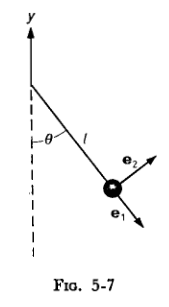
\includegraphics[scale=0.8]{p1_pendulum.png}
\end{figure}
\begin{tcolorbox}[breakable]
    \subsubsection*{a)}
    \subsubsection*{b)}
    Utilizaremos la coordenada generalizada $\theta$ para describir el movimiento, donde:
    \begin{align*}
        x &= lsin\theta \\ 
        y &= -lcos\theta + y
    \end{align*}
    derivando obtenemos:
    \begin{align*}
        \dot{x} &= l\dot{\theta}cos\theta \\
        \dot{y} &= l\dot{\theta}sin\theta + \dot{y}
    \end{align*}
    podemos encontrar la energía cinética en función de $\theta$:
    \begin{align*}
        T 
        &= \frac{1}{2}m(\dot{x}^2+\dot{y}^2) \\
        &= \frac{1}{2}m(l^2\dot{\theta}^2 + 2l\dot{\theta}\dot{y}sin\theta + \dot{y}^2) \\
        &=  \frac{1}{2}m(l\dot{\theta})^2 + \frac{1}{2}m\dot{y}^2 + ml\dot{\theta}\dot{y}sin\theta
    \end{align*}
    \subsubsection*{c)}
    Partimos de la relación:
    \begin{align*}
        \frac{\partial L}{\partial \theta} - \frac{d}{dt}\frac{\partial L }{\partial \dot{\theta}} &= 0 \\
        (ml\dot{\theta}\dot{y}cos\theta - mglsin\theta) -(ml^2\dot{\theta} + ml\ddot{y}sin\theta + ml\dot{\theta}\dot{y}cos\theta)  &= 0 \\
        -mgsin\theta - m\ddot{y}sin\theta &= ml\ddot{\theta}
    \end{align*}
\end{tcolorbox}

\section*{3.-}
\subsection*{5.9)}
Una partícula de masa $m$ se desliza, bajo la acción de la gravedad, en la superficie interior
lisa del cono invertido de la figura $5-11$ cuya ecuación es:
\[ \rho = ztan\alpha \]
\begin{enumerate}[a)]
    \item Establecer las ecuaciones de movimiento de Lagrange para la partícula.
    \item Demostrar que son posibles órbitas circulares, y hallar la velocidad de la 
    partícula en una órbita de este tipo.
\end{enumerate}
\begin{figure}[H]
    \centering
    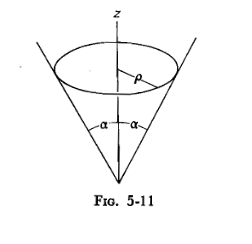
\includegraphics[scale=1]{p3_cone.png}
\end{figure}
\begin{tcolorbox}[breakable]
    \subsubsection*{a)}
    Describimos el moviminto utilizando las coordenadas generalizadas $\rho,\phi$ donde:
    \begin{align*}
        x = \rho cos\phi \\
        y = \rho sin\phi \\
        z = \rho cot\alpha
    \end{align*}
    derivando obtenemos:
    \begin{align*}
        \dot{x} &= \dot{\rho}cos\phi - \rho sin\phi \dot{\phi} \\
        \dot{y} &= \dot{\rho}sin\phi + \rho cos\phi \dot{\phi} \\
        \dot{z} &= \dot{\rho}cot\alpha
    \end{align*}
    elevando al cuadrado encontramos la energía cinética:
    \begin{align*}
        T 
        &= \frac{1}{2}m(\dot{x}^2+\dot{y}^2+\dot{z}^2) \\
        &= \frac{1}{2}m\dot{\rho}^2csc^2\alpha + \frac{1}{2}m\rho^2\dot{\phi}^2
    \end{align*}
    la energía potencial es de la forma:
    \begin{align*} 
        U 
        &= mgz \\
        &= mg\rho cot\alpha
    \end{align*}
    obtenemos las ecuaciones de movimiento recordando:
    \begin{align*}
        \frac{\partial L}{\partial q_i} - \frac{d}{dt}\frac{\partial L }{\partial \dot{q}_i} &= 0 
    \end{align*}
    aplicado a $\phi$ se tiene:
    \begin{align*}
        \frac{\partial L}{\partial \phi} - \frac{d}{dt}\frac{\partial L}{\partial \dot{\phi}} &= 0 \\ 
        0 - \frac{d}{dt}m\rho^2\dot{\phi} &= 0
    \end{align*}
    aplicado a $\rho$ se tiene:
    \begin{align*}
        \frac{\partial L}{\partial \rho} - \frac{d}{dt}\frac{\partial L}{\partial \dot{\rho}} &= 0 \\ 
        m\rho\dot{\phi^2} - mgcot\alpha - m\ddot{\rho}csc^2\alpha &= 0 
    \end{align*}
    \subsubsection*{b)}
    Veremos que una orbita de la forma:
    \begin{align*}
        \rho &= \rho_0 \\
        \phi &= w_0t
    \end{align*}
    son solucion a las ecuaciones de Lagrange, de la ultima ecuación obtenemos la restricción:
    \begin{align*}
        m\rho_0\dot{\phi}^2 &= mgcot\alpha \\
        w_0^2 &= \frac{gcot\alpha}{\rho_0} 
    \end{align*}
    la velocidad de la particula es en esta orbita es: 
    \begin{align*}
        v^2 
        &= \rho_0^2w_0^2 \\
        &= \rho_0gcot\alpha \\ 
        &= gz
    \end{align*}
\end{tcolorbox}

\section*{4.-}
\subsection*{5.10}
Considerando el sistema de partículas mostrado en la figura $5-12$:
\begin{enumerate}[a)]
    \item Escribir las ecuaciones de movimiento de Newton para cada una de las partículas, 
    en función de las variables de desplazamiento, a partir del punto de equilibrio, $x_1$ y $x_2$.
    \item Demostrar que para cualesqueira desplazamientos arbitrarios de las dos partículas, 
    la energía potencial acumulada en los resortes está dada por:
    \[ U = \frac{1}{2}k_1x_1^2+\frac{1}{2}k_2(x_2-x_1)^2 + \frac{1}{2}k_3x_2^2 \]
    \item Empleando la expresión 
    \[ T = \frac{1}{2}m_1\dot{x}_1^2+ \frac{1}{2}m_2\dot{x}_2^2 \]
    para la enrgía cinética, demostrar que las ecuaciones de Lagrange así obtenidas para 
    las variables $x_1$ y $x_2$, a partir de esta $T$ y la $U$ de la parte $b)$, concuerdan 
    con las ecuaciones de Newton halladas en la parte $a)$. ¿Cuáles supone usted que son 
    las ecuaciones de Lagrange para un sistema de partículas?    
\end{enumerate}
\begin{figure}[H]
    \centering
    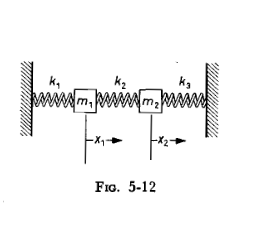
\includegraphics[scale=1]{p4_springs.png}
\end{figure}
\begin{tcolorbox}[breakable]
    \subsubsection*{a)}
    Para escribir las ecuaciones de movimiento de Newton solo hace falta notar que 
    $(x_2-x_1)$ es la distancia que se a comprimido el resorte con constante $k_2$:
    \begin{align*}
        m\ddot{x_1} &= -k_1x_1 + k_2(x_2-x_1) \\
        m\ddot{x_2} &= -k_3x_2 - k_2(x_2-x_1)
    \end{align*}
    \subsubsection*{b)}
    Obtenemos $U$ mediante la relación:
    \begin{align*}
        \bm{F}_i &= -\frac{d}{dx_i}U
    \end{align*}
    para que se cumpla en $x_1$ se debe de tener 
    \[U = -\frac{1}{2}kx_1^2+\frac{1}{2}k_2(x_2-x_1)^2\]
    para  que se cumpla para $x_2$ se debe de tener 
    \[U = -\frac{1}{2}kx_1^2+\frac{1}{2}k_2(x_2-x_1)^2-\frac{1}{2}k_3x_2^2 \]
    \subsubsection*{c)}
    Las ecuaciones de movimiento de Lagrange están dadas por:
    \begin{align*}
        \frac{\partial L}{\partial q_i} - \frac{d}{dt}\frac{\partial L }{\partial \dot{q}_i} &= 0 
    \end{align*}
    sustituyendo para $x_1$:
    \begin{align*}
        \frac{\partial L}{\partial x_1} - \frac{d}{dt}\frac{\partial L }{\partial \dot{x}_1} &= 0 \\
        -k_1x_1+k_2(x_2-x_1) - m_1\ddot{x_1} &= 0  
    \end{align*}
    sustituyendo para $x_2$:
    \begin{align*}
        \frac{\partial L}{\partial x_2} - \frac{d}{dt}\frac{\partial L }{\partial \dot{x}_2} &= 0 \\
        k_2(x_2-x_1)-k_2x_3 - m\ddot{x}_2 &= 0 
    \end{align*}
    donde podemos observar que las relaciones son las mismas obtenidas en la parte $a)$. \\
    Para describir el movimiento de un sistema de $n$ partículas en $R^k$ necesitaremos $n \cdot k$, 
    coordenadas generalizadas, donde se satisface:
    \begin{align*}
        \frac{\partial L}{\partial x_i} - \frac{d}{dt}\frac{\partial L }{\partial \dot{x}_i} &= 0 
    \end{align*}
    La energía potencial se va definir de tal forma que:
    \begin{align*}
        \bm{F_i} &= \nabla_i U \\
        \nabla_i &= \left( \frac{\partial }{\partial x_i}, \frac{\partial }{\partial x_{i+1}}, \frac{\partial }{\partial x_{i+2}} \right)
    \end{align*}
    
\end{tcolorbox}

\end{document}